\documentclass[a4paper,conference]{IEEEtran}
\usepackage{graphicx}
\usepackage{amsmath}
\usepackage{url}
\usepackage[RPvoltages]{circuitikz}
\usepackage{siunitx}
\ifCLASSOPTIONcompsoc
    \usepackage[caption=false,font=normalsize,labelfon t=sf,textfont=sf]{subfig}
\else
    \usepackage[caption=false,font=footnotesize]{subfig}
\fi

\makeatletter
\newcommand{\authornewline}{
        \end{@IEEEauthorhalign}
        \hfill\mbox{}\par\mbox{}\hfill
        \begin{@IEEEauthorhalign}
}
\makeatother

\author{
    \IEEEauthorblockN{Hernán Alejandro Silva}
    \IEEEauthorblockA{
        Facultad Regional Avellaneda\\
        Universidad Tecnológica Nacional\\
        Buenos Aires, Argentina\\
        hernansilva2002@gmail.com
    }
    \and
    \IEEEauthorblockN{Elías Ramírez}
    \IEEEauthorblockA{
        Facultad Regional Avellaneda\\
        Universidad Tecnológica Nacional\\
        Buenos Aires, Argentina\\
        ramirezelias.marcos@gmail.com
    }
    \and
    \IEEEauthorblockN{Florencia Mincone}
    \IEEEauthorblockA{
        Facultad Regional Avellaneda\\
        Universidad Tecnológica Nacional\\
        Buenos Aires, Argentina\\
        flormincone1@gmail.com
    }
    \authornewline
    \IEEEauthorblockN{Nicolás Lahorca}
    \IEEEauthorblockA{
        Facultad Regional Avellaneda\\
        Universidad Tecnológica Nacional\\
        Buenos Aires, Argentina\\
        nicolas.lahorca.k@gmail.com
    }
    \and
    \IEEEauthorblockN{Luciano Justiniano}
    \IEEEauthorblockA{
        Facultad Regional Avellaneda\\
        Universidad Tecnológica Nacional\\
        Buenos Aires, Argentina\\
        luciano.nicolas.justiniano@gmail.com
    }
}
\title{Detector de Partículas Beta}

\begin{document}
\maketitle
\begin{abstract}
    Constantemente los objetos que nos rodean emiten partículas que los sentidos
    humanos no son capaces de percibir. Estas partículas pueden ser
    perjudiciales para la salud y es necesario cuantificarlas y/o detectarlas
    para evitar o reducir la exposición a ellas. Para lograr ese objetivo, en
    este documento se presenta la realización de un dispositivo que cumpla la
    función de detectar un tipo de radiación, llamada radiación
    $\boldsymbol{\beta}$. En particular, se hará hincapié en la radiación por
    emisión de electrones, a este tipo de radiación se la conoce como radiación
    $\boldsymbol{\beta-}$. Además, se propone el análisis de su principio de
    funcionamiento, los materiales necesarios para su construcción y sus
    limitaciones.
\end{abstract}
\section{Introducción}
    El presente documento sirve como informe sobre el proyecto de fin de año de
    la asignatura Física Electrónica. Dicho proyecto se trata de un detector y
    contador de partículas beta, cubriendo de esta forma el tema radiación de
    la asignatura. Para más información sobre el proyecto, se recomienda
    visitar el repositorio del mismo que se encuentra en \cite{git_repo}.
\section{Principio de Funcionamiento}
    \subsection{¿Que son las radiaciones $\beta$?}
        Las radiaciones $\beta$ son un tipo de radiacion ionizante, la cúal se
        caracteriza por emitirse durante el proceso de desintegración o
        decaimento $\beta$. Dicho proceso puede producirse de dos diferentes
        formas.
        \begin{enumerate} 
            \item \textit{Emisión de electrones}: Un núcleo inestable de un
                átomo emite un electrón y un antineutrino, conviritiendo de esta
                manera un neutrón en un protón como \emph{Desintegración $\beta-$}.
            \item \textit{Emisión de positrones}: El núcleo inestable emite un
                positrón, es decir, un electrón cargado positivamente, junto con
                un neutrino. De esta forma se logra transformar un protón en un
                neutrón. Este proceso recibe el nombre de
                \emph{Desintegración $\beta+$}. 
        \end{enumerate}

        Generalmente, las fuentes más comunes de radiación de partículas $\beta$
        son piedras con pequeñas cantidades de uranio, y diferentes fuentes de
        potasio, como el cloruro de potasio (KCl), el cúal contiene baja
        cantidad del isótopo potasio 40 (K40), capáz de emitir partículas
        $\beta-$.

    \subsection{Formas de captar las partículas}
       El dispositivo electrónico más estudiado y utilizado para detectar la
       radiación de diferentes tipos de partículas es el diodo PIN o fotodiodo.
       Como muestra la Fig.~\ref{fig:pin}, este es similar en cuanto a
       estructura a un diodo de juntura PN, la diferencia radica en que el PIN
       tiene una zona de material semiconductor intrínseco (zona I) entre la
       zona dopada positivamente (zona P) y la zona dopada negativamente (zona
       N).\par Al ser un material semiconductor, la zona I contiene átomos de
       silicio que, al momento de ser impactados por una partícula irradiada
       debido a una fuente radioactiva, genera la rotura de los enlaces
       covalentes del átomo, produciendo un \emph{par electrón-laguna}. La
       generación de este par tiene como consecuencia un pulso de corriente de
       decenas hasta cientos de microampere que atraviesan al diodo. Esta
       corriente puede ser medida. Cuando al diodo se lo polariza en
       forma inversa (cátodo con potencial más alto que el del ánodo),
       se generan dos regiones de vaciamiento: La primera se encuentra
       localizada entre la zona P y la zona I, y la otra entre dicha zona
       intrínseca y la zona N; en estas regiones, no se encuentran portadores
       libres, sino que exisen iones fijos cargados positiva y negativamente.
       Estos iones fijos son los responsables que en dichas regiones se encuentre
       un campo eléctrico, el cúal atrapa e impulsa a los portadores, aumentando
       la intensidad de corriente eléctrica a través del diodo.
       \newpage
       \begin{figure}[!t]
           \centering
           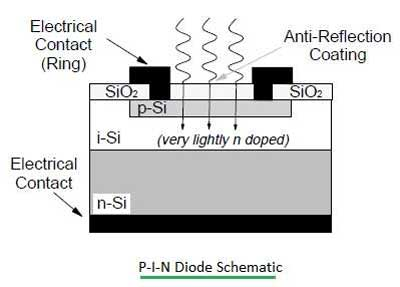
\includegraphics[width=2.5in]{img/PIN_structure.jpg}
           \caption{Corte transversal de una estructura típica del diodo PIN}
           \label{fig:pin}
       \end{figure}
    \subsection{El fotodiodo como detector de partículas $\beta$}
        La zona intrínseca explicada anteriormente es conocida como \emph{zona
        sensible}, porque es donde las partículas irradiadas impactan. Como se
        menciona en \cite{mpdi}, las zonas sensibles de los fotodiodos son
        capaces de absorber algunos tipos de radiaciones ionizantes. La
        detección de las partículas que impactan está directamente relacionada
        con la profundidad de la zona sensible del diodo; esta zona (región de
        vaciamiento) aumenta de profundidad al elevar el voltaje de polarización
        inversa del dispositivo, dicha relación responde matemáticamente a

        \begin{equation}
            \label{d_x}
            d(V) = \frac{\varepsilon_{r}\varepsilon_{0}A}{C(V)}
        \end{equation}

        \hfill \\ donde:
        \begin{itemize}
            \item d(V) es la profunidad de la zona sensible.
            \item $\varepsilon_{r}$ es la permitividad relativa del material, en este caso el Si
                (silicio).
            \item $\varepsilon_{0}$ es la permitividad del vacío.
            \item A es el área física de la zona sensible del diodo.
            \item C(V) es la capacitancia del diodo a un determinado nivel de
                voltaje de polarización inversa.
        \end{itemize}

        Este valor de profundidad permite conocer la energía cinética máxima que
        se puede detectar de una partícula. Como se mencionó anteriormente, los
        valores de interés corresponden a partículas $\beta-$ (electrones). Para
        establecer el valor de energía mencionado, es necesario conocer la
        magnitud del rango \emph{CSDA (continuos slowing down approximation)}.
        El rango CSDA es una aproximación muy cercana de la media de longitud de
        una trayectoria que recorre una partícula cargada a medida que se frena
        hasta alcanzar el reposo \cite{nist}. Para los electrones, los valores
        del CSDA están tabulados en \cite{nist}.\par 
        Para obtener una medición fiable, es necesario que el rango CSDA sea
        menor o igual que la profundidad de la zona sensible del diodo; esto es
        \begin{equation}
            R_{p} \leq d(V)
            \label{eq:range}
        \end{equation}

        \hfill \\ donde $\mathrm{R_{p}}$ es el rango CSDA.\\
        De esta forma, la energía de la partícula incidente es completamente
        disipada en el interior de la zona sensible.

    \section{Características Contructivas del Detector}
        El dispositivo a realizar para detectar las partículas tiene como foco
        ser portable y producir una señal de detección a la salida con amplitud
        observable al medir con un osciloscopio digital. Con estos objetivos
        definidos, el dispositivo estará compuesto por dos etapas:
        \begin{itemize}
            \item Etapa de detección: La opción mas documentada para la
                detección de estas partículas es el diodo PIN BPW34, que es
                posible observar en la Fig.~\ref{fig:bpw34}\subref{subfig:bpw34}; si se logra
                aislarlo completamente de la luz incidente y de interferencias
                electromagnéticas, es capaz de detectar radiaciones ionizantes
                en su zona sensible.\par
                Para aumentar la superficie total de detección, el circuito
                utiliza 4 diodos en paralelo. Esto no modifica el valor de
                profundidad de la zona sensible calculada a partir de
                (\ref{d_x}).
            \item Etapa de amplificación: Es necesario tener un nivel de ruido
                muy reducido, ya que un nivel alto escondería los picos debido a
                los impactos de las partículas. El candidato ideal que satisface
                esos requerimientos es un amplificador operacional de alta
                impedancia de entrada, como lo es la serie OPAx134 del
                fabricante Texas Instruments. A su vez, esta etapa está
                compuesta por una etapa de transimpedancia (conversión de la
                corriente de los fotodiodos en tensión) y otra de amplificación
                diferencial.
        \end{itemize}

        Ambas etapas deben tener su especificación correspondiente.

        \subsection{Etapa de detección}
            Debido a que uno de los objetivos es que el dispositivo detector sea
            portable, la alimentación del circuito es de una batería de 9 V, con
            una tensión nominal de 9,9 V. Con este valor de alimentación, el
            circuito amplificador entrega aproximadamente 8 V de polarización
            inversa a los diodos. La Fig.~\ref{fig:bpw34}\subref{subfig:c-v}
            muestra que para un nivel de tensión de 8 V de $\mathrm{V_{R}}$
            corresponde una capacitancia de aproximadamente 22 pF.\par
            Reemplazando la capacitancia (para 8 V de $\mathrm{V_{R}}$) en
            (\ref{d_x}), se obtiene

            \begin{IEEEeqnarray*}{rCl}
                d(V) & = & \frac{11,68\times 8,85\times10^{-12}\ \mathrm{F}\cdot
                \mathrm{m^{-1}}\times 7.02\ \mathrm{mm^{2}}} {22\ \mathrm{pF}} \\
                    d(V) & = & 32,98\ \mathrm{\mu m}   \\
                    d(V) & \approx & 33\ \mathrm{\mu m} 
            \end{IEEEeqnarray*}

            Esto nos indica que un electrón puede viajar como máximo 33
            $\mathrm{\mu m}$ dentro de la zona sensible, de manera tal que se
            cumpla lo expresado con anterioridad en (\ref{eq:range}).\par
            Debido a que la base de datos de \cite{nist} expresa los valores de
            rango CSDA en unidades de $\mathrm{g/cm^{2}}$, es necesario que el d(V)
            calculado esté también en dicha unidad; para esto, calculamos
            \begin{equation*}
                \sigma = \rho~t
            \end{equation*}
            donde $\sigma$ es la densidad superficial, $\rho$ es la densidad del
            silicio y t es el espesor de la zona sensible (d(V) calculado).

            \begin{figure}[ht]
                \centering
                \subfloat[] {%
                    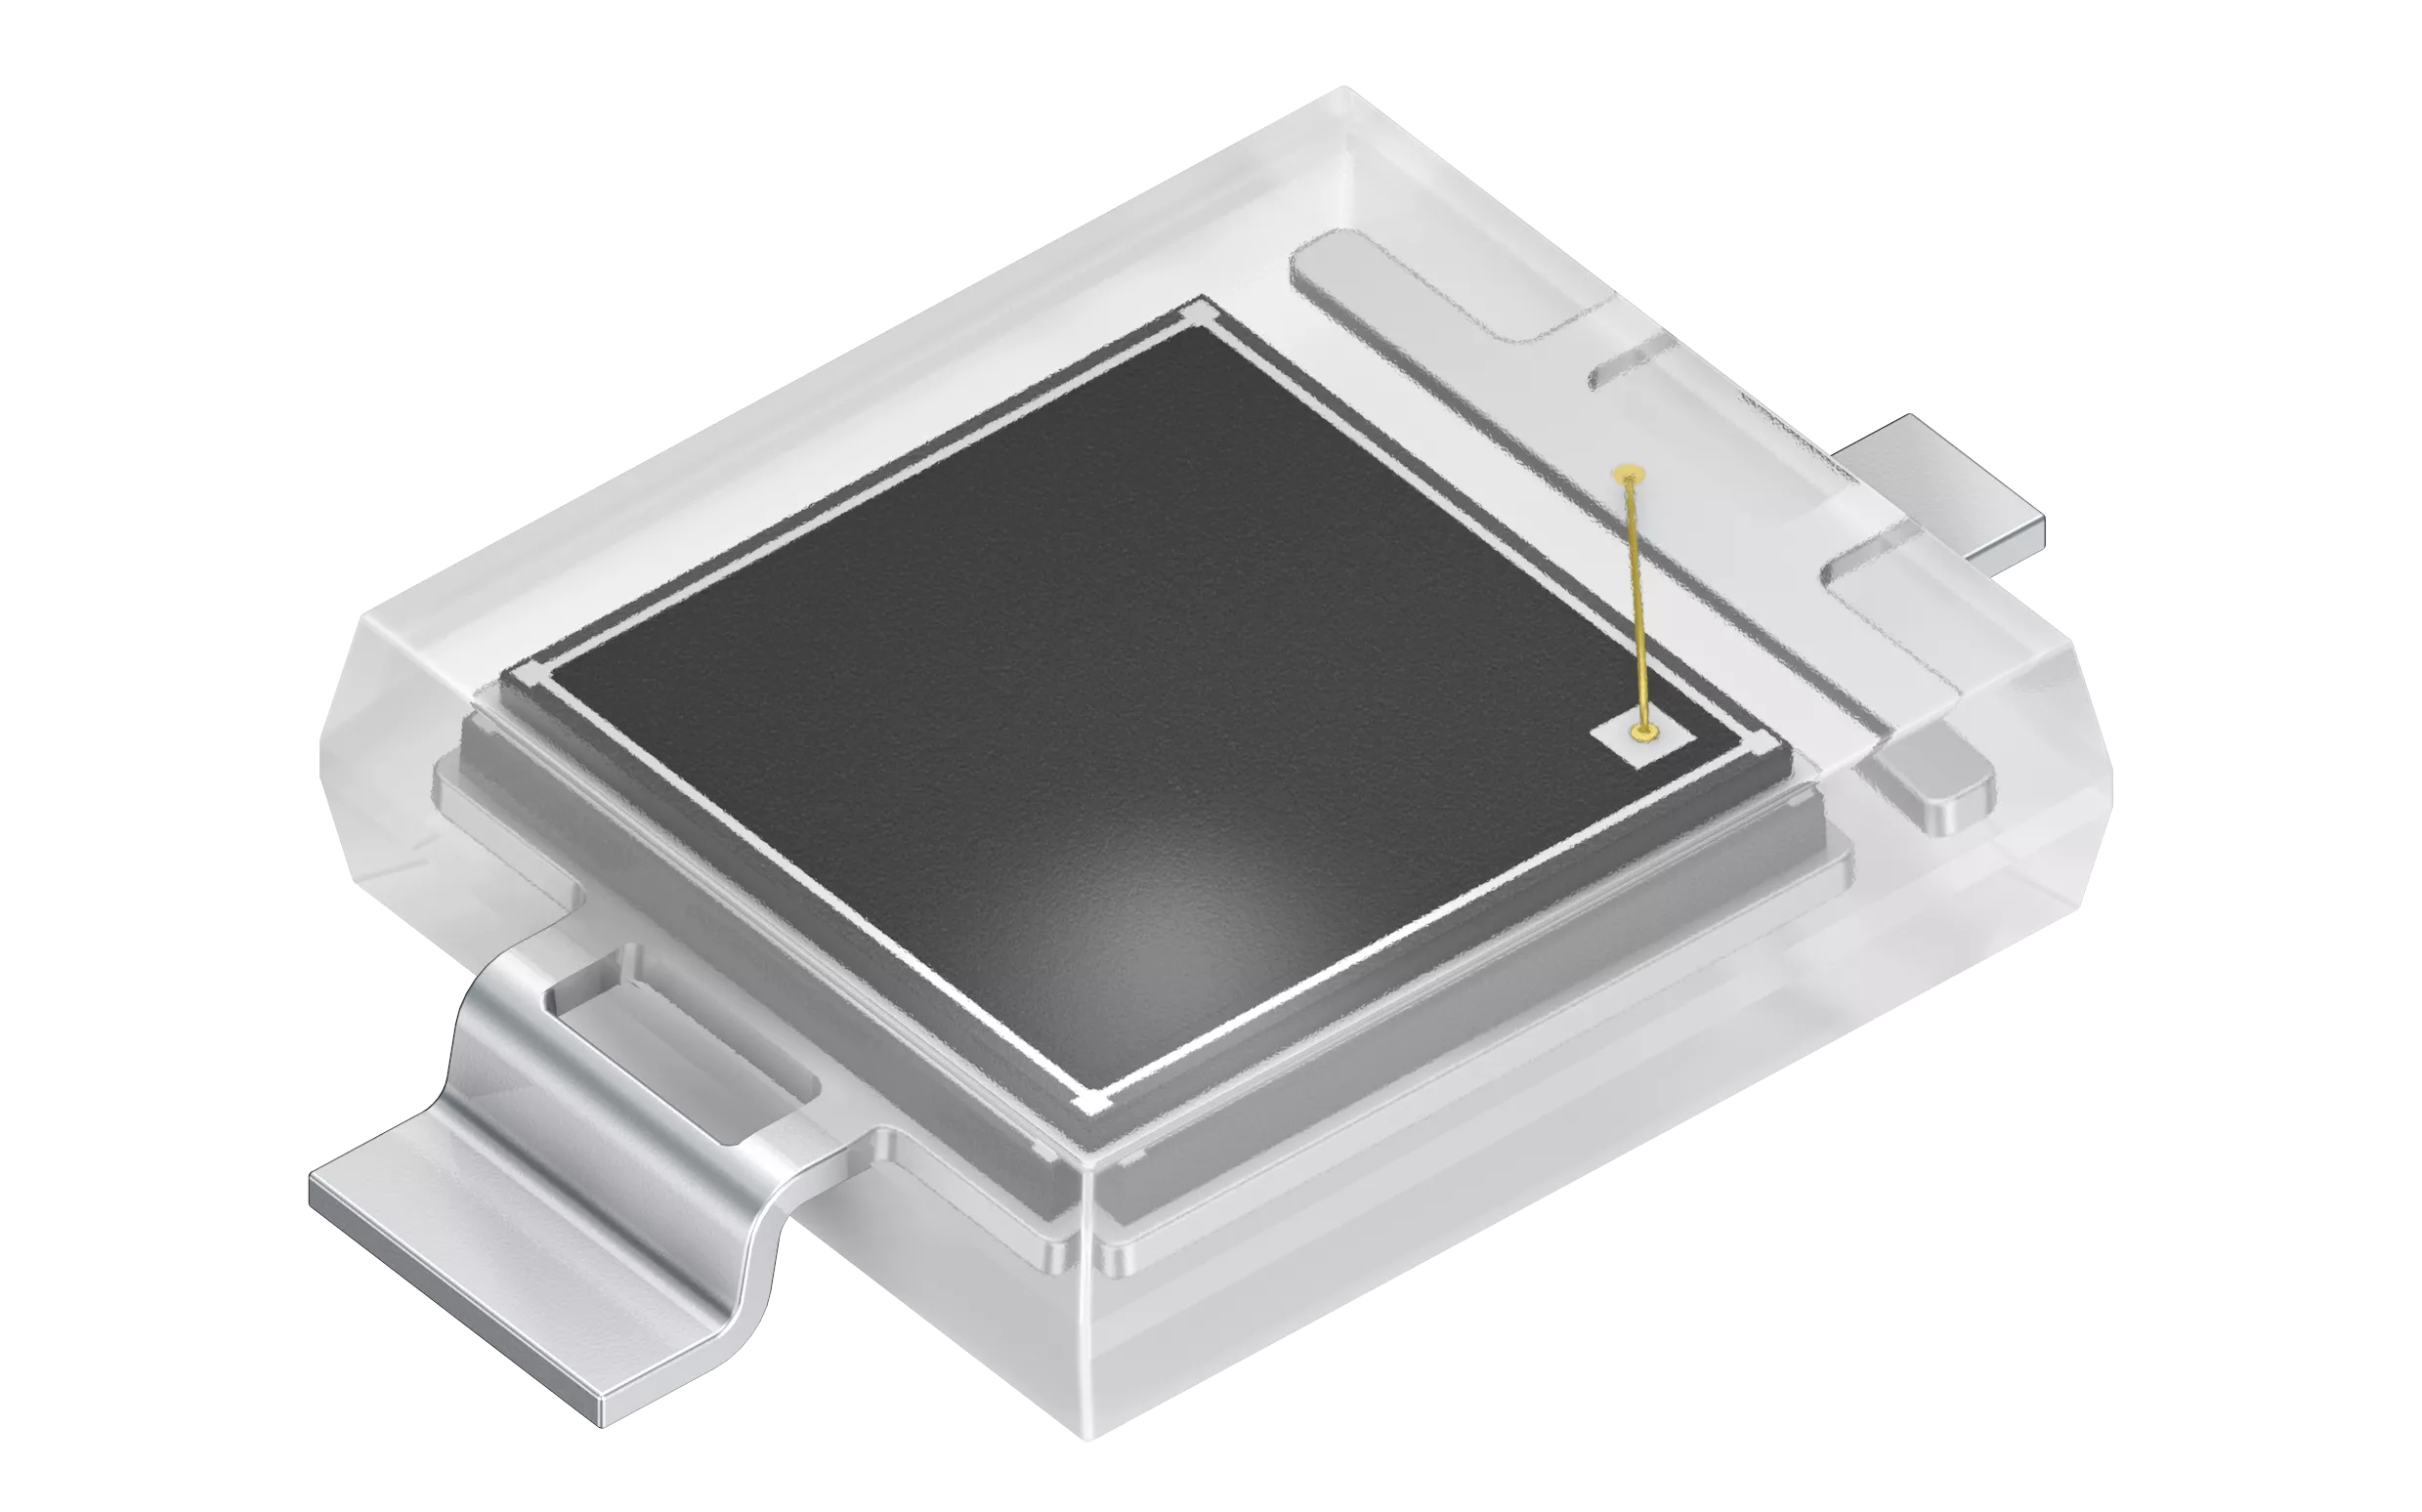
\includegraphics[width=1.5in]{img/BPW34S-ezgif.com-webp-to-png-converter.png}
                    \label{subfig:bpw34}
                }
                \hfil
                \subfloat[] {%
                    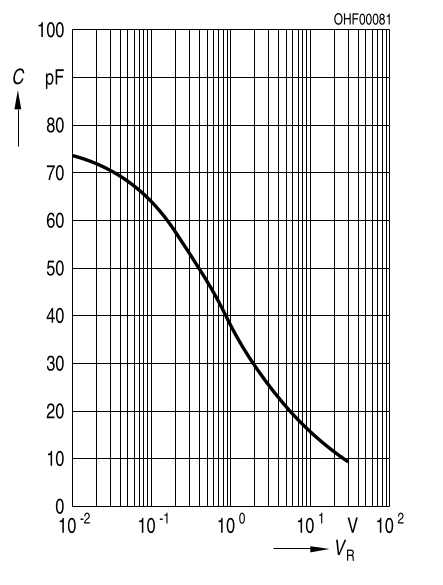
\includegraphics[width=1.5in]{img/C-V.png}
                    \label{subfig:c-v}
                }
                \caption{Fotodiodo BPW34S de la marca Osram. (a) Imágen real del
                fotodiodo. (b) Curva característica C-V del BPW34S}
                \label{fig:bpw34}
            \end{figure}

            Para 33 $\mathrm{\mu m}$, esto es
            \begin{IEEEeqnarray*}{C} %deberia usar \begin{equation} con \begin{split}
                \sigma=\rho~t\\
                \sigma= 2,32\ \mathrm{g\cdot cm^{-3}}\ \times \ 0,0033\
                \mathrm{cm}\\%
                       = 7,6\times 10^{-3}\ \mathrm{g\cdot cm^{-2}}
            \end{IEEEeqnarray*}

            En la base de datos de \cite{nist} es posible observar que para el
            Si, la energía cinética máxima del electrón para un rango de
            $7,6\times 10^{-3}\ \mathrm{g\cdot cm^{-2}}$ es 60 KeV.

            Con el fin de anular interferencias electromagnéticas externas y la
            luz del ambiente, el circuito se ubica dentro de un gabinete
            estanco de aluminio.
        \subsection{Etapa de amplificación}
            El amplificador operacional, cuyas descripciones se explicó
            anteriormente, consta de 2 etapas; ambas se pueden ver en la
            Fig.~\ref{fig:circ}.
            \begin{itemize}
                \item Etapa de transimpedancia (primer etapa): Para transformar
                    los picos de corriente en picos de voltaje es necesario
                    utilizar un primer amplificador en configuración
                    transimpedancia; su característica fundamental es que la
                    corriente generada en los diodos (decenas de microampere)
                    atraviesa una resistencia de realimentación de valor grande,
                    generando, por ley de Ohm, una caida de tensión en ella. A
                    la salida del primer amplificador tendremos
                    \begin{equation*}
                        V_{out1} = V_{ref1} - I_{D}\ R_{fb}
                    \end{equation*}
                    donde $\mathrm{V_{ref1}} = V\ R1/(R1+R2)$ es la tensión de referencia del
                    primer amplificador; su valor tiene que ser 8 V y se logra a
                    partir del divisor de voltaje entre las resistencias R1 y R2
                    de la Fig.~\ref{fig:circ}. $\mathrm{I_{D}}$ es la corriente
                    de los diodos y $\mathrm{R_{fb}}$ es la resistencia de
                    realimentación (\emph{feedback}), equivalente a R3 en
                    la Fig.~\ref{fig:circ}
                \item Etapa de amplificación (segunda etapa):
                    $\mathrm{V_{out1}}$ es de valor de tensión muy débil, por
                    ello es necesario amplificar la salida de la primer etapa.
                    Esto es posible mediante un segundo amplificador que toma
                    como entrada $\mathrm{V_{out1}}$.
            \end{itemize}

            Al utilizar 2 amplificadores operacionales (uno por etapa), es
            necesario adoptar el amplificador OPA2134 de la línea OPAx134
            previamente mencionada. 
            \tikzset{every picture/.style={/tikz/font=\normalsize}}



            \begin{figure}[!t]
                \centering
                \ctikzset{bipoles/length=7mm, amp symbol font={\footnotesize}}
                \begin{circuitikz}[american, font=\footnotesize, transform shape,
                    scale=0.46]
    %\ctikzset{diodes/scale=0.5}
                    \centering
                    \draw
                    (0,0) to[photodiode,name=D1] (0,5)
                    node[above left=5pt](D1label) at (D1) {$D_{1}$}
                    node[below left=3pt] at (D1) {BPW34S}
                    (0,0) node[ground, scale=2] {}

                    (2,0) to[photodiode,name=D2] (2,5)
                    node[above left=5pt] at (D2) {$D_{2}$}
                    node[below left=3pt] at (D2) {BPW34S}
                    (2,0) node[ground, scale=2] {}

                    (4,0) to[photodiode,name=D3] (4,5)
                    node[above left=5pt] at (D3) {$D_{3}$}
                    node[below left=3pt] at (D3) {BPW34S}
                    (4,0) node[ground, scale=2] {}

                    (6,0) to[photodiode,name=D4] (6,5) coordinate(vd4)
                    node[above left=5pt] at (D4) {$D_{4}$}
                    node[below left=3pt] at (D4) {BPW34S}
                    (6,0) node[ground, scale=2](d4gnd) {}

    % muevo el cursor desde gnd de D4 hasta donde termina la pata de D4 creo una linea desde el D4 con long = 1
                    ++(0,5)
                    to[short] ++(2,0)

                    node[op amp, anchor=-] (opamp) {}
                    (0,5) -- (opamp.-)
                    (opamp.up) ++ (.2,0) node[right=2pt] {U1}
                    (opamp.down) ++ (.2,0) node[below=2pt, right=2pt] {OPA2134}
                    (opamp.down) -- node[ground, scale=2] {} ++(0,0)
                    (opamp.down) node[below=1pt, right] {$-$}
                    (opamp.up) node[above=2pt, right=-0.5pt] {$+$}
                    (opamp.+) -- ++(0,-1) coordinate(VD1)
    % primer divisor
                    to[R] node[above=35pt, right=4pt] {$R_{2}$} node[above=25pt,
                    right=4pt] {\SI{15}{\kilo\ohm}} (VD1 |- d4gnd) node[ground, scale=2] {}
                    (VD1) to[short,*-] ++(.75,0)
                    to[R, l=$R_{1}$, a=\SI{4.7}{\kilo\ohm}] ++(.75,0) to[short,-*] ++(.75,0) node[right] {+9 $\mathrm{V}$} % Resistencia del divisor
                    (VD1) ++(0,-.5) to[short, *-] ++(-1.15,0) coordinate(cR2)
                    to[C] node[above=5.5ex, right=1ex] {$C_{3}$} node[above=3ex, right=.5ex] {\SI{100}{\nano\farad}} (cR2 |- d4gnd) node[ground, scale=2] {}
                    (opamp.up) %-- ++(0,.5) coordinate(V+C1)
                    to[C, l=$C_{2}$, a=\SI{100}{\nano\farad}] ++(0,1) node[vcc](vcc) {} node[above right=.5pt] {+9~V}
                    (vd4) to[short, *-] ++(0,2)
                    to[R, l=$R_{3}$, a=\SI{10}{\mega\ohm}] ++(4.5,0) coordinate(r3_out1)
                    (opamp.out) -- (r3_out1 |- opamp.out) coordinate(vout1_node1)
    % capacitor en paralelo a R3
    %(r3_out1) to[short, *-] ++(0,1)
                    to[short,*-] (vout1_node1 |- r3_out1)
                    (vout1_node1 |- vout1_node1) to[C, l=$C_{4}$,
                    a=\SI{100}{\nano\farad}] ++(1.5,0)
                    to[R, l=$R_{4}$, a=\SI{1}{\kilo\ohm}] ++(2.5,0) coordinate(vin2-)
    % segunda etapa
                    node[op amp, anchor=-] (opamp2) {}
                    (opamp2.up) ++ (.2,0) node[right=2pt] {U2}
                    (opamp2.down) ++ (.2,0) node[below=2pt, right=2pt] {OPA2134}
                    (opamp2.up) to[C, l=$C_{2}$, a=\SI{100}{\nano\farad}] ++(0,1.2) node[vcc](vcc) {} node[above right=.5pt] {+9~V}
                    (opamp2.down) -- node[ground, scale=2] {} ++(0,0)
                    (opamp2.down) node[below=1pt, right] {$-$}
                    (opamp2.up) node[above=2pt, right=-0.5pt] {$+$}

                    (opamp2.+) -- ++(0,-1) coordinate(VD2)
                    to[R] node[above=35pt, right=4pt] {$R_{7}$} node[above=25pt,
                    right=4pt] {\SI{10}{\kilo\ohm}} (VD2 |- d4gnd) node[ground, scale=2] {} 
                    (VD2) to[short,*-] ++(.75,0)
                    to[R, l=$R_{6}$, a=\SI{10}{\kilo\ohm}] ++(.75,0) to[short,-*] ++(.75,0) node[right] {+9 $\mathrm{V}$} % Resistencia del segundo divisor
                    (VD2) ++(0,-.5) to[short, *-] ++(-1.15,0) coordinate(cR7)
                    to[C] node[above=5.5ex, right=1ex] {$C_{6}$} node[above=3ex, right=.5ex] {\SI{100}{\nano\farad}} (cR7 |- d4gnd) node[ground, scale=2] {}

                    (vin2-) ++(-.5,0) coordinate(vin2-_new)
                    to[short, *-] (vin2-_new |- r3_out1)
                    to[R, l=$R_{5}$, a=\SI{100}{\kilo\ohm}] ++(4.5,0) coordinate(r5_out1)
                    (opamp2.out) -- (r5_out1 |- opamp2.out) coordinate(vout2_node1)
                    to[short,*-] (vout2_node1 |- r5_out1)
    % out, final del circuito
                    (vout2_node1) to[short, *-o] ++(1,0) node[above] {Output}
                    (r3_out1) to[short, *-] ++(0,1.5) to[C, l=$C_{1}$, a=\SI{5}{\pico\farad}] ++(-4.5,0)
                    to[short, -*] ++(0,-1.5)
                    (r5_out1) to[short, *-] ++(0,1.5) to[C, l^=$C_{5}$, a=\SI{10}{\pico\farad}] ++(-4.5,0)
                    to[short, -*] ++(0,-1.5)
                    ;
                \end{circuitikz}
%                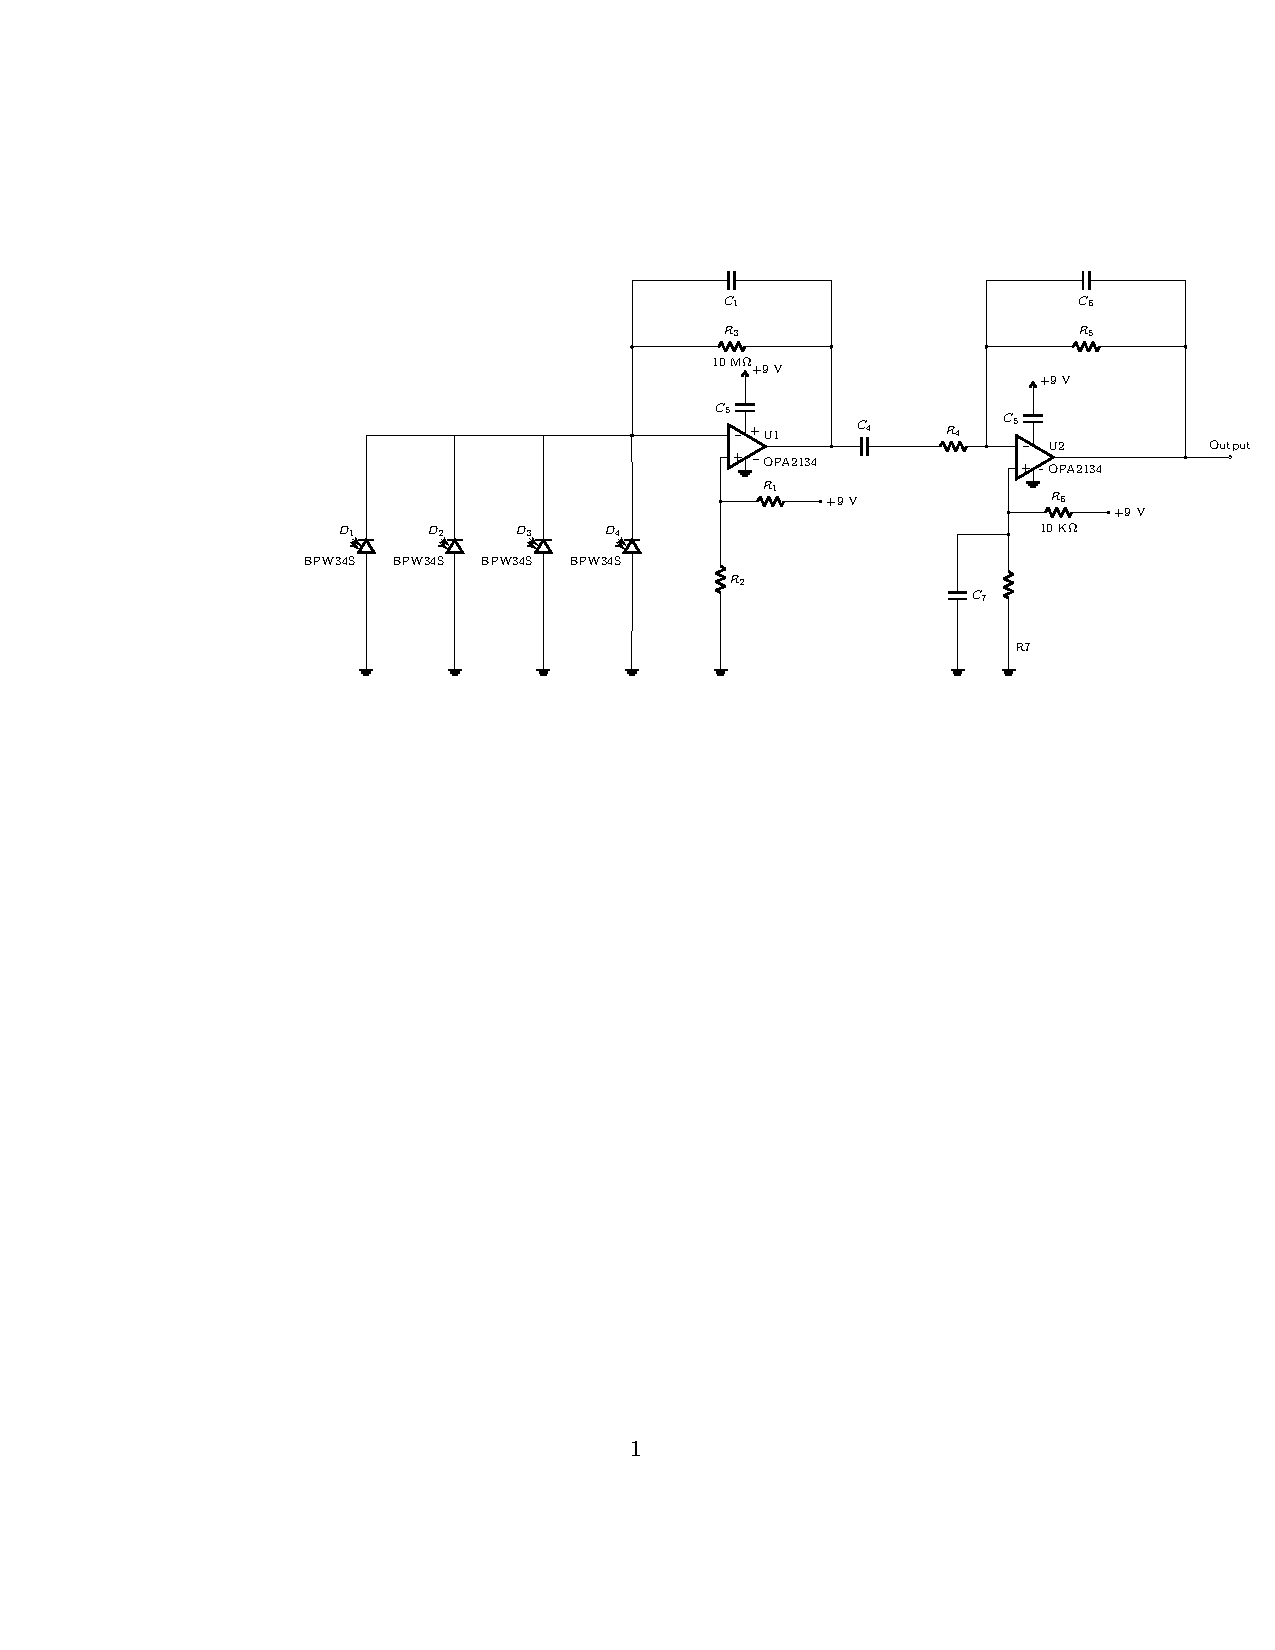
\includegraphics[width=\linewidth]{circuito.pdf}
                \caption{Circuito completo}
                \label{fig:circ}
            \end{figure}

            \begin{figure}[!t]
                \centering
                \subfloat[] {%
                    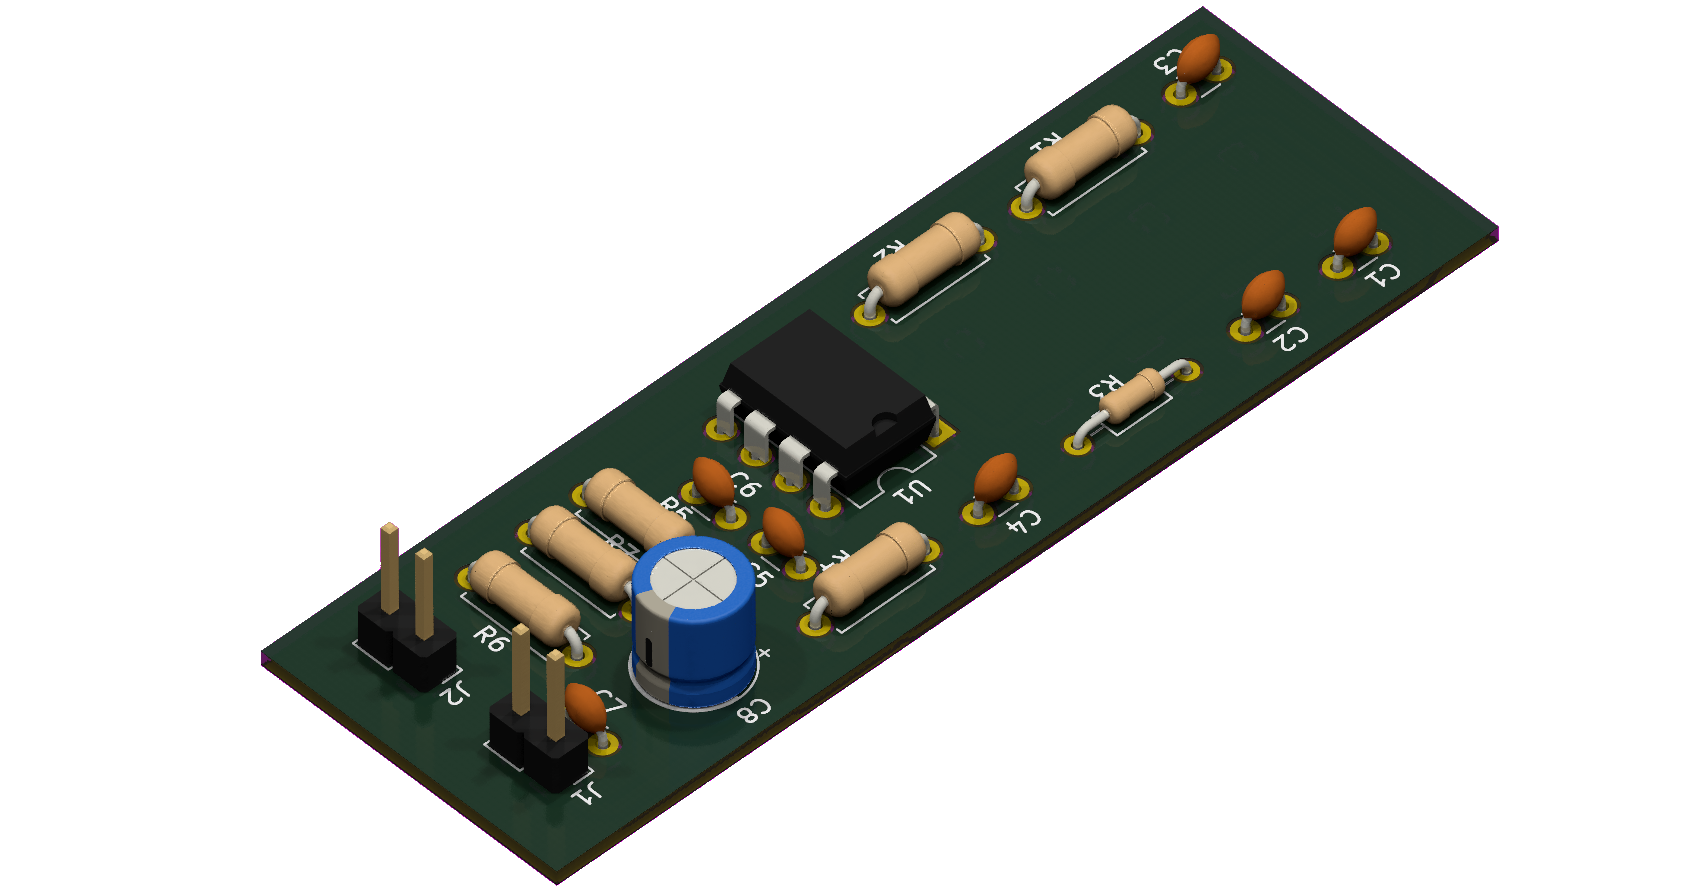
\includegraphics[width=2in]{img/pcb_front.png}
                    \label{subfig:pcb_front}
                }
                \hfil
                \subfloat[] {%
                    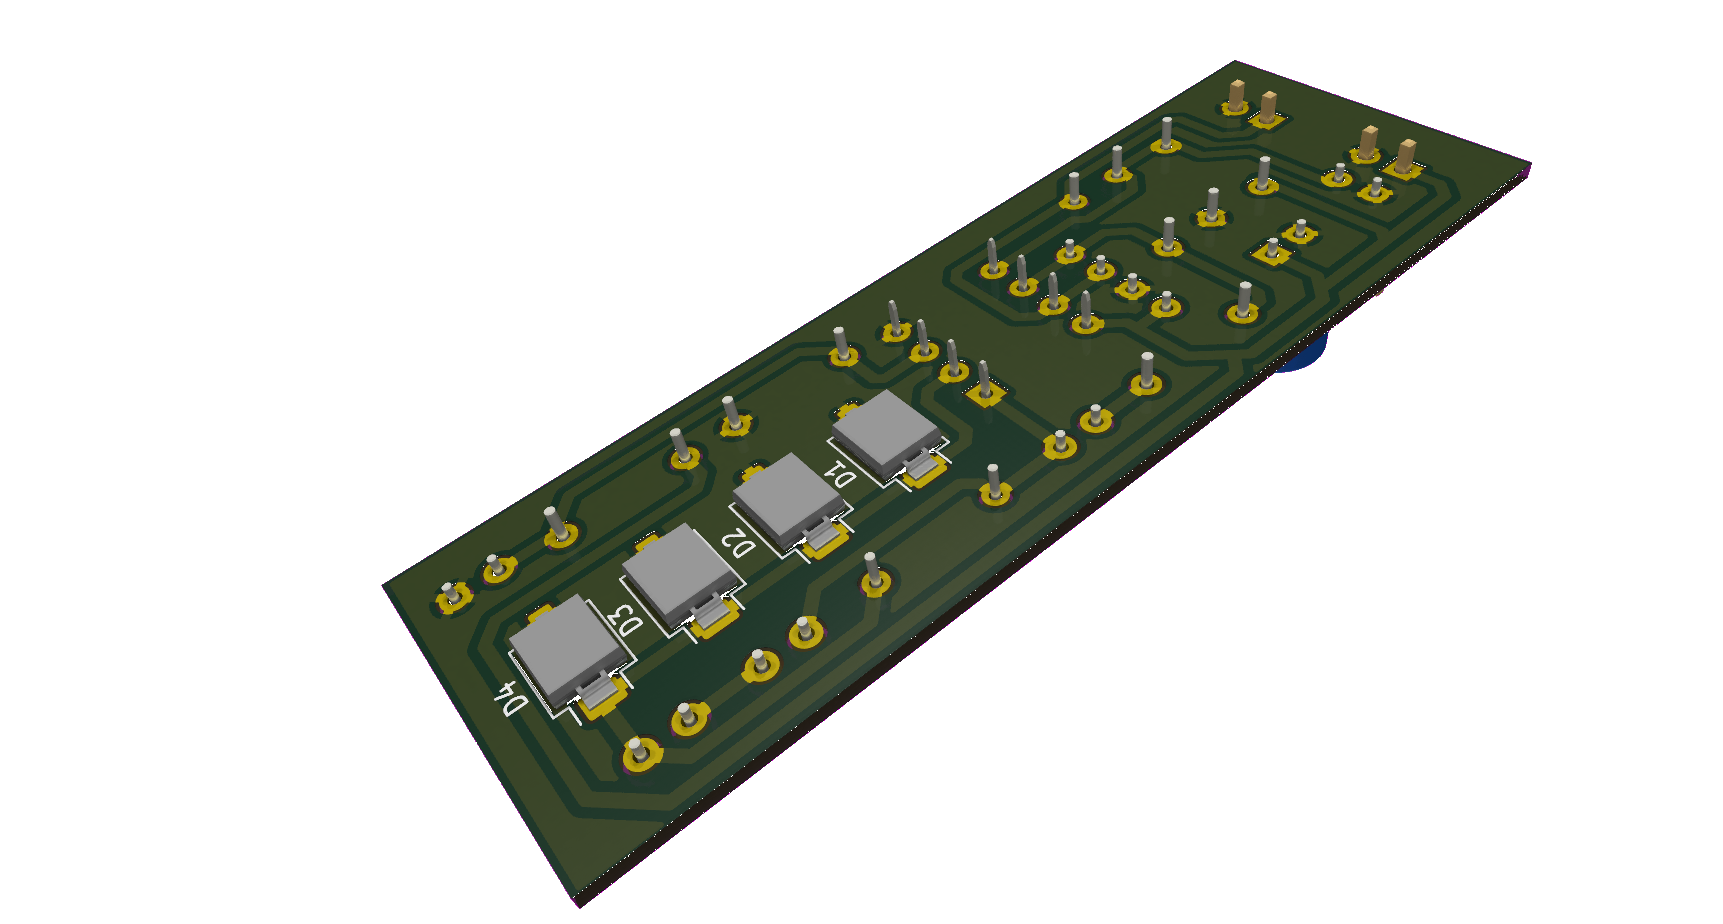
\includegraphics[width=2in]{img/pcb_rear.png}
                    \label{subfig:pcb_rear}
                }
                \caption{Modelado 3D del PCB. (a) Parte frontal, (b) parte
                posterior}
                \label{fig:pcb}
            \end{figure}


\section{Limitaciones del Diseño}
    Las limitaciones o posibles mejoras del diseño actual son las siguientes
    \begin{enumerate}
        \item Niveles de energía cinética detectables: Como se ha expresado
            anteriormente, el nivel máximo de energía medible es 60 KeV, lo cúal
            es un valor relativamente bajo para partículas $\beta-$; partículas
            con más energía no serán medidas correctamente. Esto es debido
            principalmente al área efectiva de detección (área física de la zona
            sensible de los diodos) y al valor de capacitancia del diodo para
            $\mathrm{V_{R}}$ dado. Una mejora viable para este problema es el
            aumento del voltaje de alimentación, de manera tal que aumente
            $\mathrm{V_{R}}$.

        \item Nivel de ruido: el capacitor C4 que se puede observar en la
            Fig.~\ref{fig:circ} tiene un papel fundamental en los niveles de
            ruido de la salida del circuito. Empíricamente se pudo advertir
            que utilizando un valor de 22 pF en lugar de 5 pF, las mediciones  
            de los picos fueron más limpias.
    \end{enumerate}

\section{Conclusiones}
    Aunque el diseño de detectores de partículas con fotodiodos requiere de un nivel de
    precisión muy grande para evitar capacitancias parásitas y obtener el menor
    nivel de ruido posible montado en la señal de salida, es posible realizar
    mediciones de radiación $\beta-$ utilizando un amplificador operacional
    basado en JFET en configuración transimpedancia. 
% Las malditas referencias. TODO: Sacar este comment.
\bibliographystyle{IEEEtran}
\bibliography{refs}
\nocite{*}
\end{document}
